\documentclass[a4paper ]{article}
\usepackage{graphicx}
\usepackage[letterpaper, landscape, margin=2in]{geometry}
\geometry{
	paper=a4paper, % Change to letterpaper for US letter
	inner=0.5cm, % Inner margin
	outer=0.5cm, % Outer margin
	bindingoffset=0.01cm, % Binding offset
	top=0.5cm, % Top margin
	bottom=0.5cm, % Bottom margin
	%showframe, % Uncomment to show how the type block is set on the page
}
\usepackage[utf8]{inputenc}
%\usepackage{natbib}

\begin{document}
- - -

\vspace{50mm}
\begin{center}
{\Huge \textsc{\textbf{Instrucciones del Experimento}}}\\
\end{center}

\begin{center}
\textit{\huge Estudios en Detección de Señales - Tesis de Licenciatura}\\
\bigskip
\end{center}

\begin{center}
\textit{\huge Adriana F. Chávez De la Peña}\\
\end{center}

\begin{center}
\vfill
\textit{\huge adrifelcha@gmail.com}\\
\end{center}
\newpage

\begin{center}
{\LARGE \textbf{Pantalla de Bienvenida}}\\
{\large \textsc{(igual para ambos experimentos)}}\\
-  -  -  -  -  -  -  -  -  -  -  -  -  -  -  -
\smallskip
\end{center}
%\begin{center}
%{\LARGE \textit{Experimento }}\\
%\end{center}
\vspace{3mm}
\begin{figure}[th]
\centering
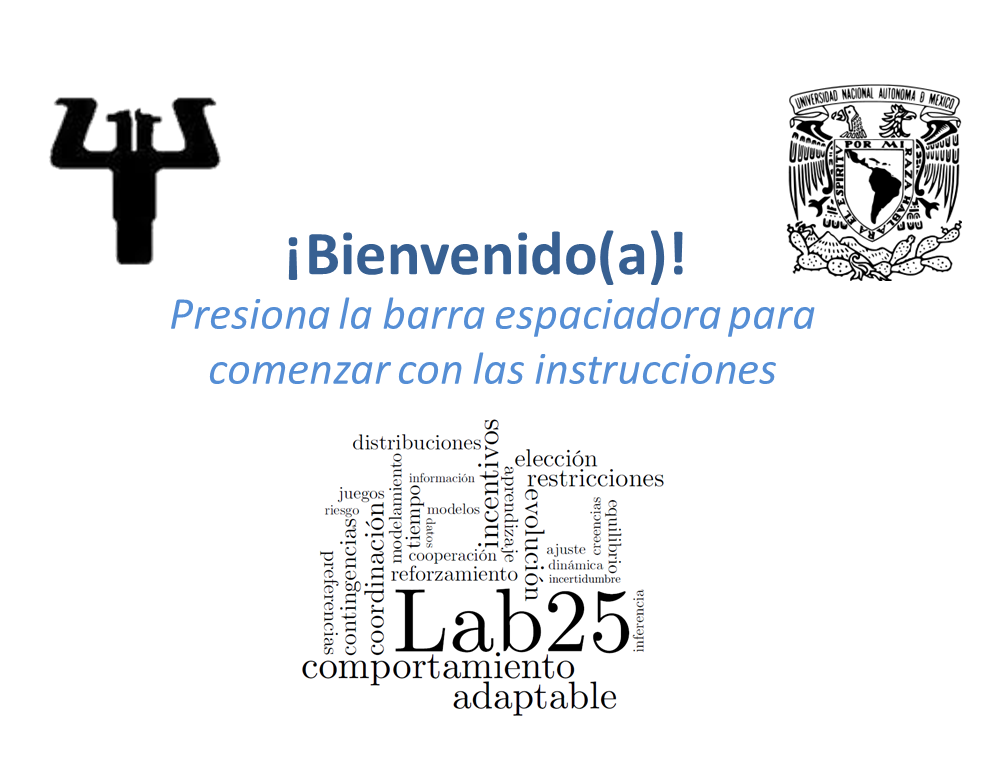
\includegraphics[width=.7\textwidth]{Figures/Inst_Bienvenido} 
\end{figure}
\clearpage






\begin{center}
{\LARGE \textbf{Instrucción Principal}}\\
{\large \textsc{(Experimento 1)}}\\
-  -  -  -  -  -  -  -  -  -  -  -  -  -  -  -
\smallskip
\end{center}
%\begin{center}
%{\LARGE \textit{Experimento }}\\
%\end{center}
\vspace{3mm}
\begin{figure}[th]
\centering
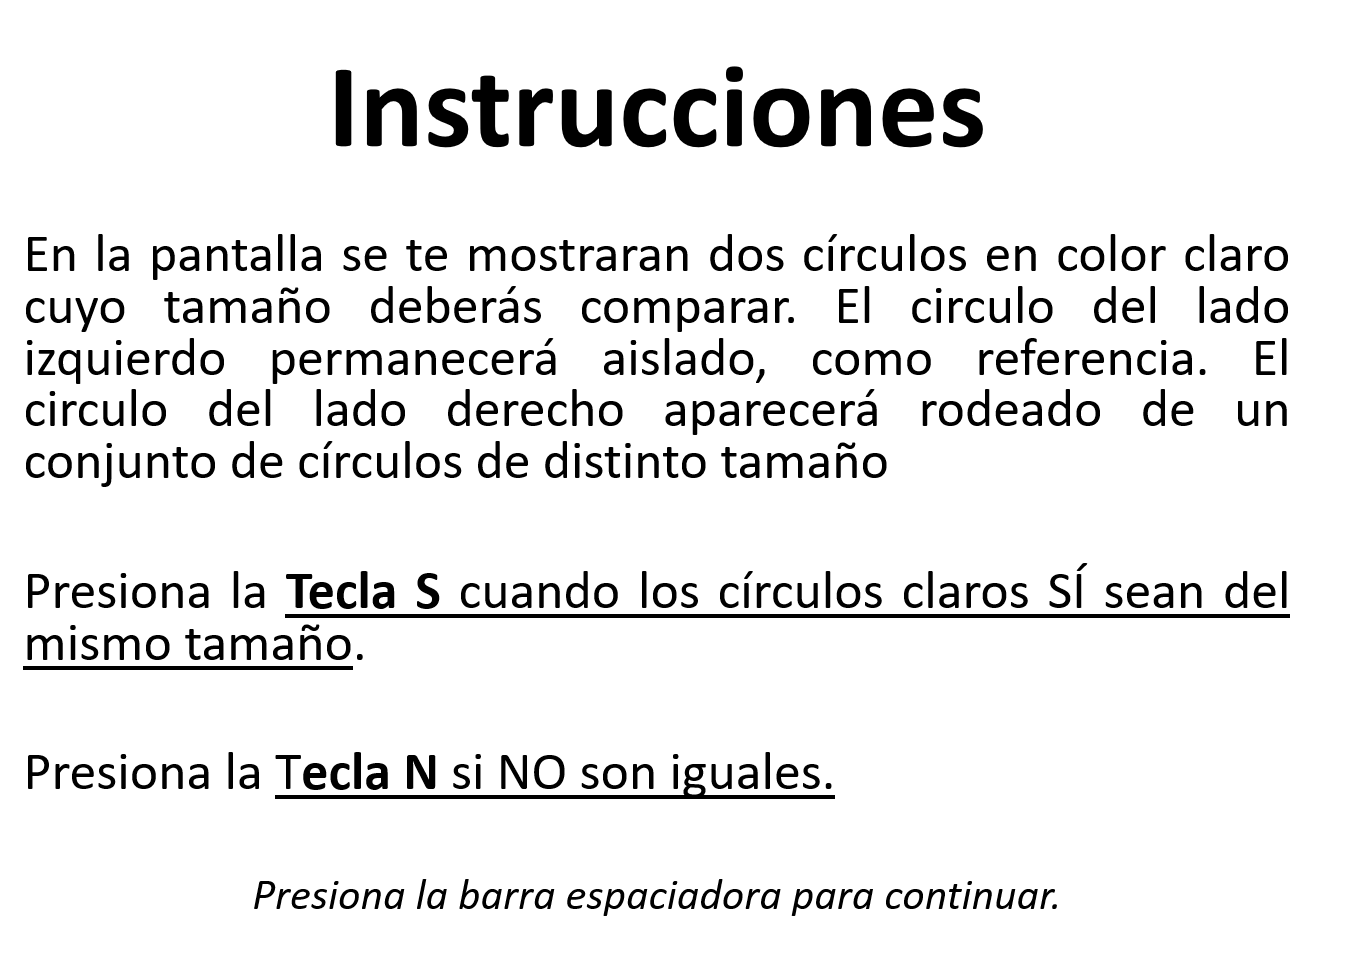
\includegraphics[width=0.7\textwidth]{Figures/Inst_1b} 
\end{figure}
\clearpage






\begin{center}
{\LARGE \textbf{Instrucción Principal}}\\
{\large \textsc{(Experimento 2)}}\\
-  -  -  -  -  -  -  -  -  -  -  -  -  -  -  -
\smallskip
\end{center}
%\begin{center}
%{\LARGE \textit{Experimento }}\\
%\end{center}
\vspace{3mm}
\begin{figure}[th]
\centering
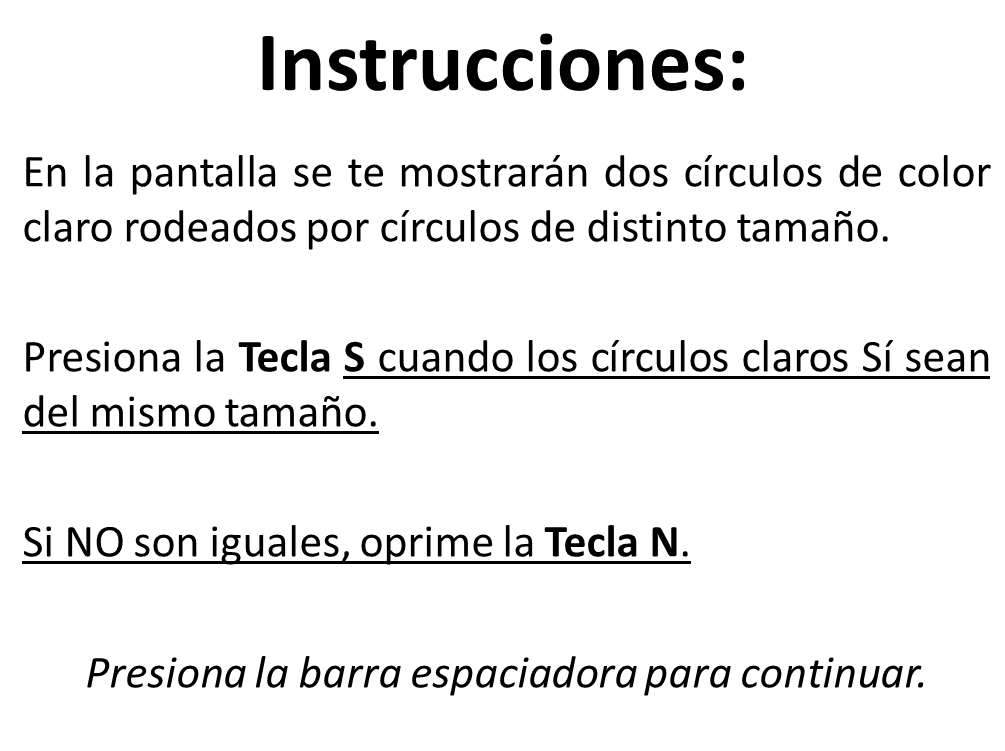
\includegraphics[width=0.7\textwidth]{Figures/Inst_1} 
\end{figure}
\clearpage





\begin{center}
{\LARGE \textbf{Ejemplo}}\\
{\large \textsc{(Experimento 1)}}\\
-  -  -  -  -  -  -  -  -  -  -  -  -  -  -  -
\smallskip
\end{center}
%\begin{center}
%{\LARGE \textit{Experimento }}\\
%\end{center}
\vspace{3mm}
\begin{figure}[th]
\centering
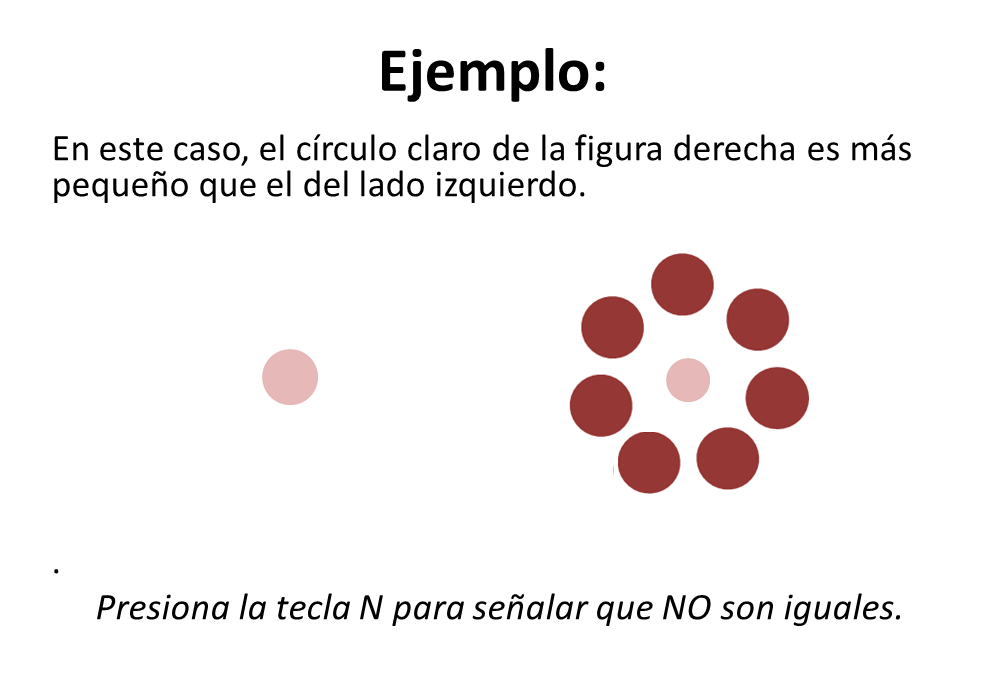
\includegraphics[width=0.7\textwidth]{Figures/Inst_Ex} 
\end{figure}
\clearpage







\begin{center}
{\LARGE \textbf{Ejemplo}}\\
{\large \textsc{(Experimento 2)}}\\
-  -  -  -  -  -  -  -  -  -  -  -  -  -  -  -
\smallskip
\end{center}
%\begin{center}
%{\LARGE \textit{Experimento }}\\
%\end{center}
\vspace{3mm}
\begin{figure}[th]
\centering
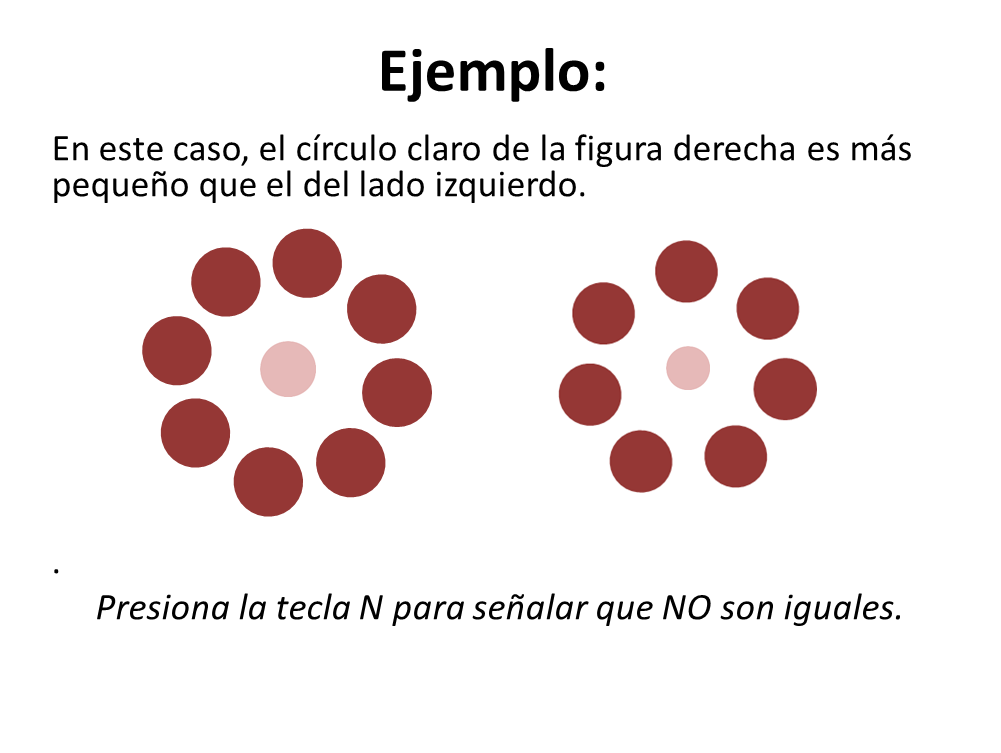
\includegraphics[width=0.7\textwidth]{Figures/Inst_Ex2} 
\end{figure}
\clearpage







\begin{center}
{\LARGE \textbf{Instrucción Escala de Confianza}}\\
{\large \textsc{(Igual para ambos experimentos)}}\\
-  -  -  -  -  -  -  -  -  -  -  -  -  -  -  -
\smallskip
\end{center}
%\begin{center}
%{\LARGE \textit{Experimento }}\\
%\end{center}
\vspace{3mm}
\begin{figure}[th]
\centering
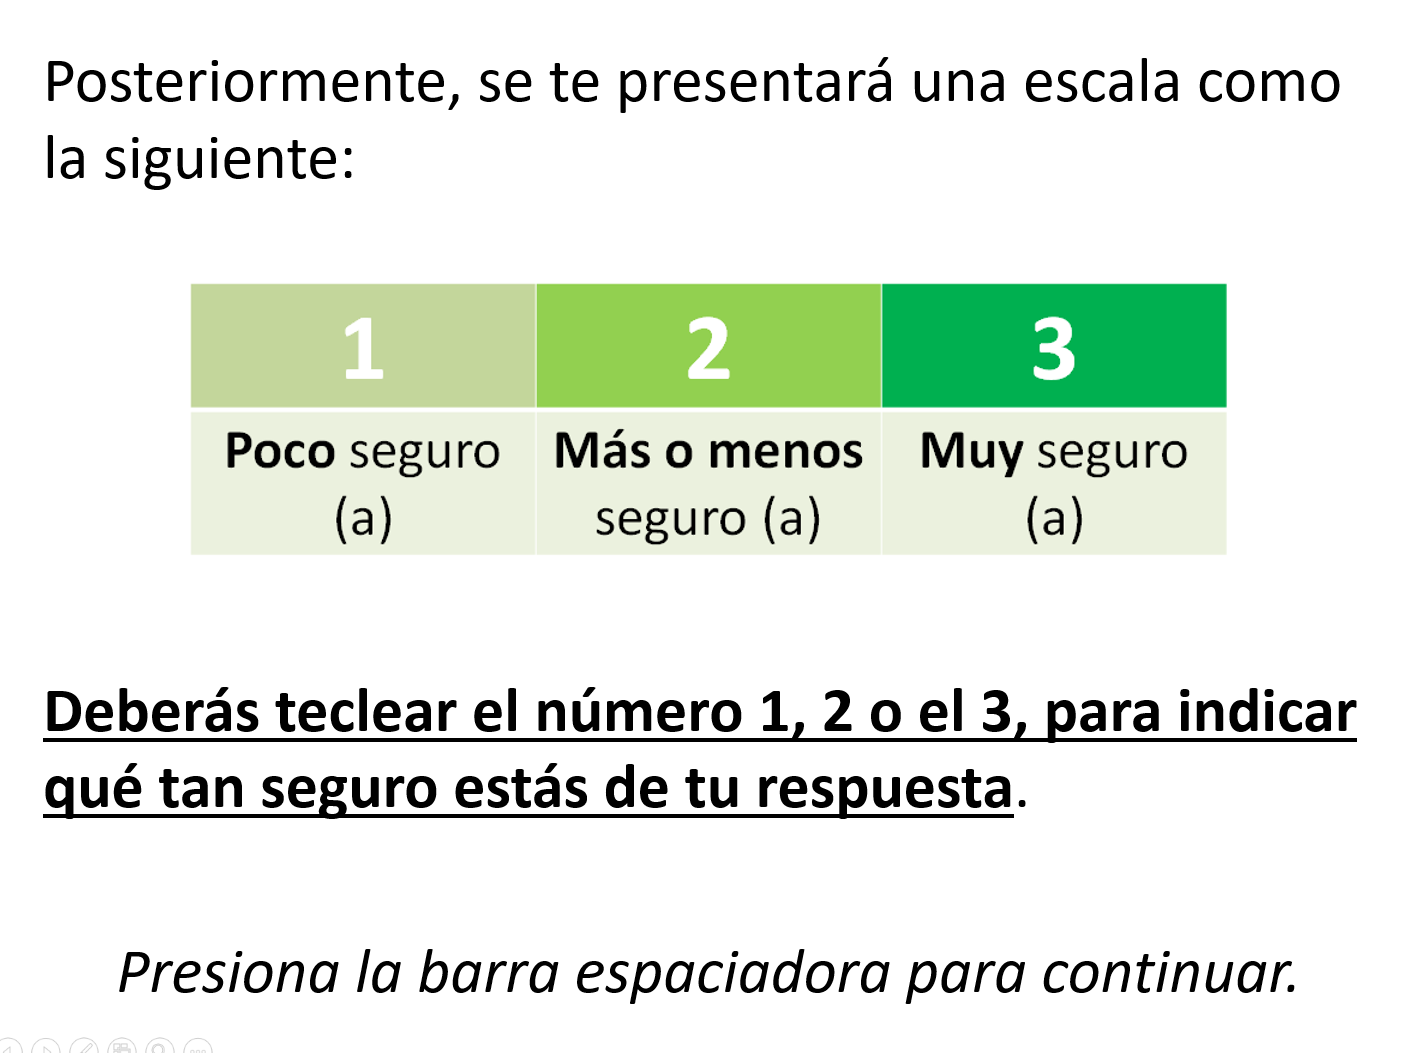
\includegraphics[width=0.7\textwidth]{Figures/Inst_Regla}  
\end{figure}
\clearpage








\begin{center}
{\LARGE \textbf{Especificaciones}}\\
{\large \textsc{(Igual para ambos experimentos)}}\\
-  -  -  -  -  -  -  -  -  -  -  -  -  -  -  -
\smallskip
\end{center}
%\begin{center}
%{\LARGE \textit{Experimento }}\\
%\end{center}
\vspace{3mm}
\begin{figure}[th]
\centering
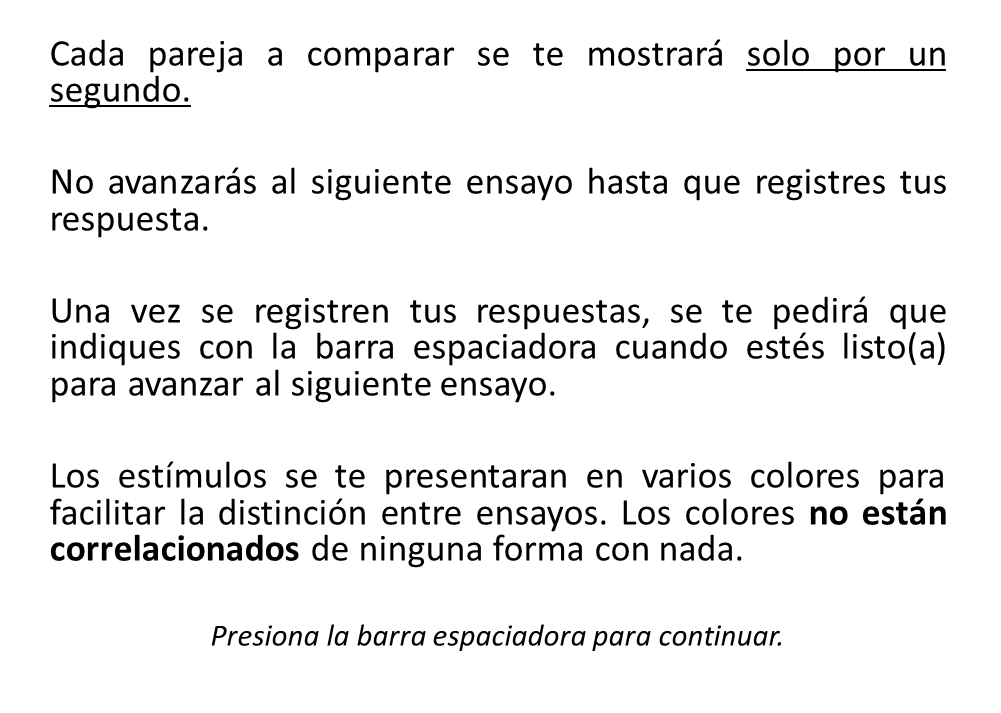
\includegraphics[width=0.7\textwidth]{Figures/Inst_3}  
\end{figure}
\clearpage










\begin{center}
{\LARGE \textbf{Recordatorio Final}}\\
{\large \textsc{(Igual para ambos experimentos)}}\\
-  -  -  -  -  -  -  -  -  -  -  -  -  -  -  -
\smallskip
\end{center}
%\begin{center}
%{\LARGE \textit{Experimento }}\\
%\end{center}
\vspace{3mm}
\begin{figure}[th]
\centering
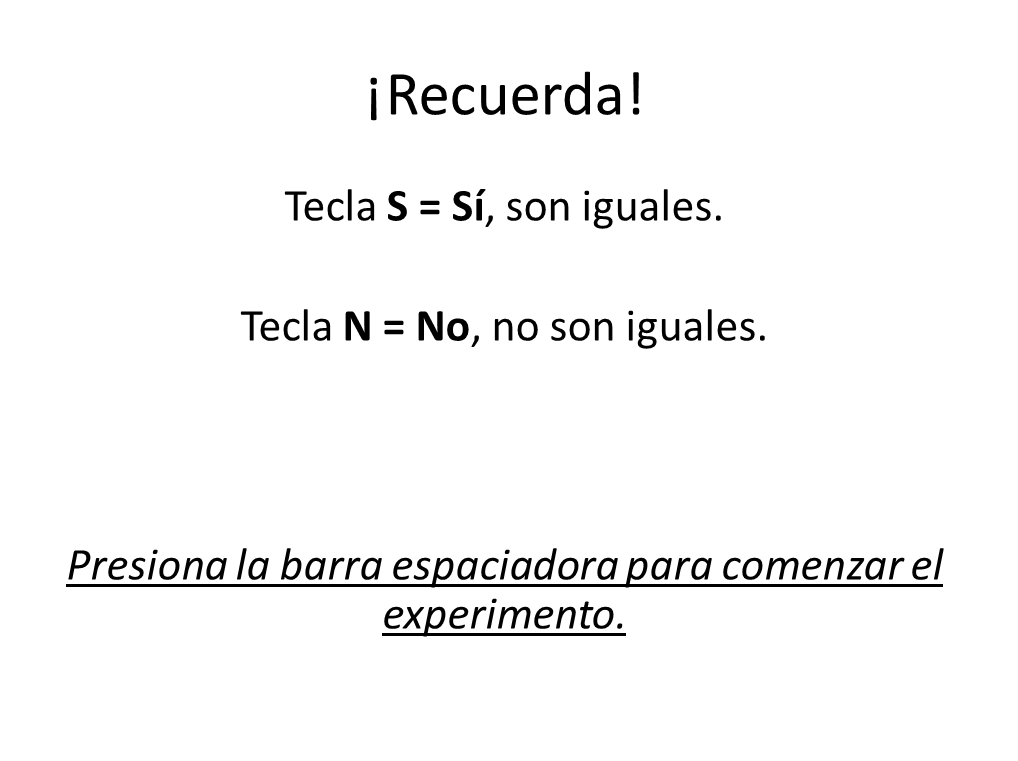
\includegraphics[width=0.7\textwidth]{Figures/Inst_4} 
\end{figure}
\clearpage



\end{document}